\documentclass[fontset=none]{ctexart}
\ctexset{fontset=windows}   %指定字体库为windows
\usepackage{fancyhdr}
\setlength{\headheight}{13pt}  % 调整页眉高度
\usepackage{float}
\usepackage{mathtools}
\usepackage[left=3cm,right=3cm,top=2.5cm,bottom=2.5cm]{geometry}
%\usepackage{graphicx}  %插入图片
\usepackage{epstopdf}
\usepackage{stmaryrd}
\usepackage{subcaption} 
\usepackage{wrapfig}   %设置环绕图片
\pagestyle{fancy}
\fancyhf{} % 清空默认页眉页脚
\fancyhead[L]{QQ:17950026}
\fancyhead[R]{作者:姜鱼}
\fancyhead[C]{兼听则明,偏听则暗}
\fancyfoot[C]{\thepage}

%\usepackage{lmodern}
\makeatletter
\renewcommand{\thesubsection}{\arabic{subsection}} % 仅显示subsection自身的数字
\renewcommand{\maketitle}{
  \begin{flushleft} % 整体左对齐
    {\huge\bfseries \@title \par} % 标题
    \vspace{0.5em}
    {\large \bfseries \textit{作者:} \@author \par} % 作者(添加自定义文字)
    \vspace{0.5em}
    {\large\bfseries \textit{日期:}\@date}% 日期(调整格式)
  \end{flushleft}
  \thispagestyle{empty} % 可选:隐藏页眉页脚
  \vspace{1cm} % 标题块后间距
}
\makeatother

\begin{document}
\title{对于不同均值含义的探索}
\author{姜鱼}
\date{\today}
\maketitle
\kaishu

\subsection{线性均值与调和均值}

首先来看线性的均值:

\lishu
例题1:现有一直线上由四个点A、B、C、D划分的三个线段 $L_1$、$L_2$、$L_3$ ,定义其平均长度满足 $ 3 \bar{L} = L_1 + L_2 + L_3$ ,则 $\bar{L} = \frac{L_1 + L_2 + L_3}{3}$ 。

\kaishu
我们对其直接求均值的思路,很符合朴素的对均值概念的直觉,但是若问题略作改变呢?

\lishu
例题2:现有一起点A和终点B,其距离为L。一物体以速度 $v_1$ 匀速由A走向B,再以速度 $v_2$ 由B返回A。求整个过程的平均速度 $\bar{v}$ 。

显然答案不再是$v_1+v_2$那么简单的了。我们可以从速度的定义角度出发,设$A\to B$所需时间为$t_1$, $B\to A$ 所需时间为 $t_2$ , $\bar{v}=\frac{2L}{t_1 + t_2}$ 。 因为$v_1 = \frac{L}{t_1}$,$v_2 = \frac{L}{t_2}$故可见 $\bar{v} = \frac{2v_1v_2}{v_1+v_2}$。

\kaishu
这是为什么呢?

本质还是要追溯到$v$的定义上来。对于位移L,它不取决于我们如何定义,而是直接对独立成果的描述,在无任何特性干扰的情况下,其均值必然是线性相加的。而速度$v$的定义并非L那般直接,而是以$\frac{L}{t}$的方式定义。这是一个分式,一个变量v可以拆分为分式上下两个结构构成,所以我们考察v需要综合L和t整体来看。

这个问题中,往返两个过程的L是固定的,由于往返时间不同,才导致速度不同。我们以处于分母结构中的变量为线索,将整体过程拆分为 $t_1\text{与}t_2$ 两个路径。相对于线性均值可将L直接拆分为 $L_1\text{和}L_2$ ,速度的均值则是将分母处的t拆分为$t_1\text{和}t_2$。如果我们只关注分母结构,将速度取倒数来看,则会发现速度式满足$\frac{2}{\bar{v}} = \frac{1}{v_1}+\frac{1}{v_2}$或$$2\cdot\frac{t_1+t_2}{2L} = \frac{t_1}{L} + \frac{t_2}{L}$$

其当与线性均值无异。

所以无非是直接取平均,亦或者对分母结构取平均罢了。若并非以分母结构为线索,譬如以不同速度等时间地经过两段路程,我们以分子结构处L为线索取均值,依然有$\bar{v}=\frac{v_1 + v_2}{2}$。

于是我们索性定义一种名为\textbf{倒数空间}的视角,通过取倒数的方式实现由线性空间到倒数空间的变换,再进一步考察导数空间中的量被线性地拆分为了不同部分,并将其整合,求平均。
\begin{wrapfigure}[6]{r}{0.3\textwidth} % {r} 表示右侧,{0.3\textwidth} 为图片宽度
  \centering
  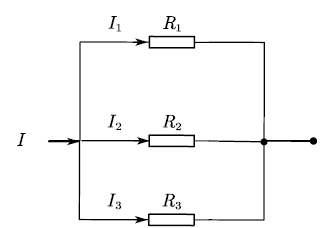
\includegraphics[width=0.3\textwidth]{2025-03-22_152403.png} % 宽度略小于容器宽度
  \label{1}
\end{wrapfigure}

\lishu
例题3:对于并联的三个电阻,求其等效的电阻值。

并联意味着每个电阻的两端都连接着同一个节点,电压相同,且电流分别流过三个路径。

可观察到电阻的定义$R = \frac{U}{I}$与之前的模型较为相似,在倒数空间中,电流被分到三条路径并行流过。只是此次我们并非求其均值,而是对所有并联路径的电阻进行求和,故式子发生一些微妙的变化:$$\frac{1}{R_\text{总}}=\frac{I_1+I_2+I_3}{U}=\frac{I_1}{U}+\frac{I_2}{U}+\frac{I_3}{U}=\frac{1}{R_1}+\frac{1}{R_2}+\frac{1}{R_3}$$注意$R_\text{总}$处的分子并不是3而是1,也正是说并非将其拆分为三个$\frac{1}{\bar{R}}$相加,或认为$$\frac{1}{R_\text{总}}=\frac{1}{\bar{R}}+\frac{1}{\bar{R}}+\frac{1}{\bar{R}}=\frac{3}{\bar{R}}=\frac{1}{R_1}+\frac{1}{R_2}+\frac{1}{R_3}$$即为此意。

\kaishu
我们可以从期望的角度出发:一个整体被拆分为不同部分,每一部分虽各有差异,但是整体却具有一种统一的性质。我们求均值,实际上是综合一个整体后,求一个能够等价替换每一个部分的量。这个量可以近似地代表整体的每个部分,所以实际上期望这个词,才应该更符合我们真正所求的目标,而均值,或者说平均,更多倾向于描述求期望的“手段”。

均值,是求出不同部分的总和,再均分为n份分配给每个部分。引用此例,一来是用并联模型强化对倒数空间的认知,二来也想强调虽然我们需要从整体考虑均值,但是均值只为每条并联分路的等价期望值,并非直接等于所有路径的总和。

此外,我们需要关注“路径”这一概念。电路并联的例子可以很生动地展示电流的路径。其实对于一般分式来说,其对于现实的含义往往都有“比率”的意义在:我们考虑微积分中取极限的比率$y=\frac{dy}{dx}$,其往往揭示了y随x变化而变化的速率。对于单变量x,其路径方面的含义并不显著,而对于多变量函数$y=f(a,b)$来说,其两个求导路径$\partial y/\partial a\text{和}\partial y/\partial b$是显著不同的。甚至对于含参t的单变量函数$y=f(x)$,若$x=g(t)$,其一阶导虽具有形式不变性:$dy=f'(x)dx=g'(t)dt$,但也是因为有约束方程而存在链式法则。如至于二阶导,则会由于求导路径的问题,失去微分的形式不变性:$d^2y=f''(x)dx^2\ne g''(t)dt^2$。这可以体现求导路径的意义,由此体现分式的性质,进而可以增强对调和均值的路径分配属性的理解。

对于倒数空间中所取得的平均数叫做\textbf{调和平均}数:$$H = \frac{n}{\frac{1}{a_1} + \frac{1}{a_2} + \dots + \frac{1}{a_n}}$$

再举一个工程应用中出现的例子以说明调和均值的模型。(其实思考这个问题的过程正是诱发姜鱼写这篇文章的原因)

\lishu
例题4:在AI学习的工程中,我们需要给学习结果进行评价。AI会对一类事情进行预判,我们将机器给出的判断与现实做对比,并通过综合的评价,进一步指导机器学习的方向,使机器的预测结果尽可能贴近现实结果。
首先给出如下定义:

\begin{wrapfigure}[5]{r}{0.33\textwidth} 
  \centering
  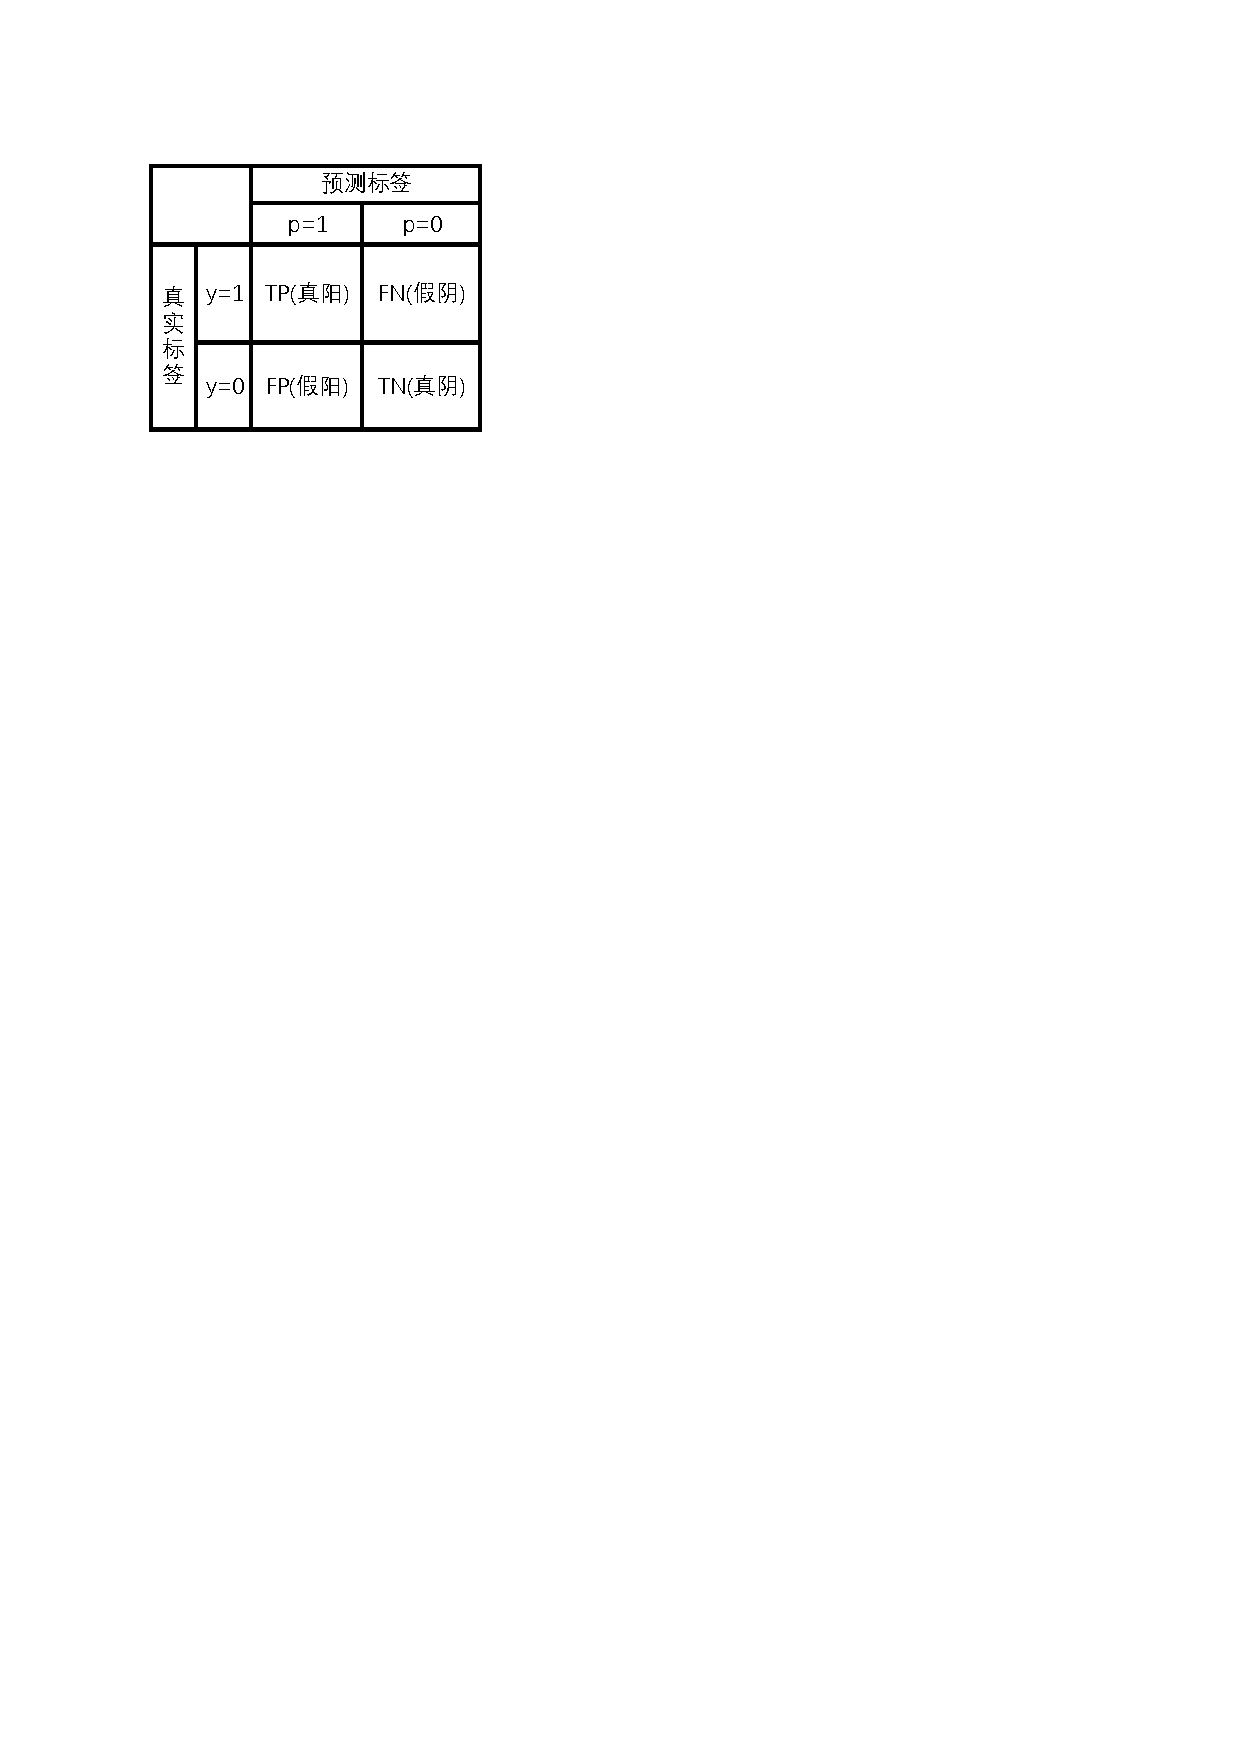
\includegraphics[width=0.33\textwidth]{2.pdf}
  \label{2}
\end{wrapfigure}

\textbullet现实:真(true)

\textbullet现实:假(false)

\textbullet预测:真(positive)—— 阳性

\textbullet预测:假(negative)—— 阴性


\textbullet 准度:阳性案例中真实案例的比例
	$$\text{准度}=\frac{TP}{TP+FP}$$

\textbullet 召回率:真实案例中阳性案例的比例
	$$\text{召回率}=\frac{TP}{TP+FN}$$

准度和召回率都是很有用的指标,我们既希望在真实案例中召回更多阳性案例,又希望在阳性案例中保持较高的真实案例的准度。所以我们需要定义一个新的指标$F$用以代表准度和召回率对结果的平均作用效果。

用A表示准度,R表示召回率,仔细观察可发现A和R都以TP作为分子,显然考虑的对象是一致的。其差异所在分母,分母的意义在于所选的样本环境不同。二者其一是从\textbf{预测样本}的正例中寻找TP,另一个是从\textbf{现实样本}的真例中寻找TP。从两个样本出发的两条路径导向结果,恰如电路中电流从不同路径实现由电势A降低电压U到达电势B的节点。

那么我们进而对这两条环境路径进行并联考虑,在倒数空间中计算它的线性均值。其结果就当以调和均值的结果体现:$$\frac{2}{F}=\frac{1}{A}+\frac{1}{R}$$或$$F=\frac{2AR}{A+R}$$

\kaishu
此外,还有诸如圆锥曲线中常见的极点极线问题,其涉及调和点列之类数学领域的概念。

\subsection{几何均值}

\kaishu
我们常说分类加法,分步乘法。之前的模型,无论线性均值还是调和均值,都是通过分类加法计算的。调和均值无非是预处理了目标数的结构,将其分为分子分母两份,然后进一步处理分母的线性均值。其实质上离线性均值相差不大。

接下来我们要处理一类全新的模型,是增长率类模型。准确来说是分步类模型,目标值往往由分步乘积构成。

\lishu
例题5:在生态学中,种群的增长常呈现指数模型。求某生物种群两年的平均增长率,设该生物种群每年以不同速率增长:

- 第一年:环境适宜,增长率为50\%(种群数量增长至原来的 1.5倍);

- 第二年:资源受限,增长率为-20\%(种群数量下降至原来的 0.8倍);

起点值记为$1$,第一步(经过一年后):种群数量数量为 $y_1 = 1.5×1=1.5$,第二步(经过第二年后):种群的数量 $y_2 = 0.8×y_1 = 0.8×1.5=1.2$ ,故增长后的种群数量为$1.2$。若存在一个统一的年均增长率$r$,使其等效代替每一步增长,从而令$(1+r)×(1+r)=1.2$,我们可解得$r = \sqrt{2}-1 \approx 0.095 = 95\%$。即为平均增长率,亦是几何均值。

\kaishu
对于同一系统的分步作用效果,每一步都是将作用系数乘以系统的当前值。类似于等比数列:$a_{n+1}=k×a_n$,所以整体是类似于指数增长的。但是每一步的k可以有所不同,所以结果为$$a_1\cdot k_1\cdot k_2\dots \cdot k_n$$
对于$n$个不同过程的$k_i$,我们寻找n个等价的k填充每一个步骤,即为求其几何均值。定义为:
$$k=\sqrt[n]{k_1k_2\cdots k_n}$$

可以看出,核心的思路没有变:“拆!”线性均值将事物拆为不同部分,调和均值在倒数空间拆为不同路径,几何均值将事物拆成不同步骤。那么在此类比之下,对于几何均值而言,有没有同“线性空间”和“倒数空间”一般的什么空间呢?

有的兄弟,有的,当然是我们的\textbf{对数空间}了。

首先考虑对数有什么性质——摘掉指数。对于等比数列$a_n = q^n$,$ln a_n = n\cdot ln q$。可见取对数后,在对数的外边可以得到其步骤的数量n,在对数里可以得到每一步的作用量$q$。现考虑用这个等比数列去实现等效地取代原有分步乘法,可得到几何:$$n\ln q=\ln q_1+\ln q_2+\cdots +\ln q_n$$这正是几何均值的对数表达式。

通过对数可以使乘法化为加法的性质,我们用ln包裹住了每一步的作用量因子$q_i$,并将其转化为线性求和的方式。故而可视几何均值为对数空间中的线性均值,这依然有助于凸显分步的协同作用。

\lishu
例题6:某股票连续两天涨跌幅为+10\%和-5\%,如何计算“平均波动”?

在线性空间中计算均值:\( \frac{10\% - 5\%}{2} = 2.5\% \),但实际总回报为 \( 1.1 \times 0.95 -1 = 4.5\% \)。

显然这是几何均值模型:\( \sqrt{1.1 \times 0.95} -1 \approx 2.23\% \),准确反映复合效应。

而在对数空间中,我们把步骤拆到每个ln中,依然可以以线性均值的方式计算: $$ \text{均值} = \frac{ln(1.1) + ln(0.95)}{2} \approx 0.022 \quad \Rightarrow \quad e^{0.022} \approx 1.0223 \, (2.23\%)$$

\kaishu
通过上面的例题,我们发现:如果说倒数空间尚且能想象(至少以有理的方式构造),那么对数空间涉及到无理函数或者超越函数了。既过于抽象,又使步骤更加繁琐,何必多此一举。那么定义这种东西有什么意义呢?有的兄弟,还是有的。

\lishu
例题7:信息论中,我们可以以“是”或“否”的方式传达两个判断信息,如果进行两步的判断,显然可以传达四个不同信息,例如\{是,是\}、\{是,否\}、\{否,是\}、\{否,否\}为四组不同信息。

用0记录否,用1记录是,则可以将逻辑信息编码为二进制代码。将上述四组信息用二进制编码表示,则分别为11、10、01、00。用n个是或否传递信息,转换为的二进制数称为n位二进制编码,其包含的独立信息量个数为$2^n$。

可见,这是一种高效的压缩信息的方式:逆向思维来说,我们可以将一群指数级别的$2^n$个信息压缩为只有$log_22^n=n$位的二进制编码进行打包传递。对于小于$2^n$个信息的包来说,其最少所需的位数另说,但是最多所需的位数依然不超过n位。所以对于任意数量M的信息,其所需的二进制编码长度为将$log_2M$向上取整的位数。

如果M并非恰好为$2^n$,将其取对数后将是无理数,我们虽然很难精确地,恰好地用二进制编码存储此大小的信息量,但是我们可以在理论上视其为最小信息量。

以上我们了解了二进制编码和信息量与指数形式的关系,接下来考虑信息量与概率的关系。如果一个包含所有事件的总样本 $\Omega$ 中,包含许多等可能不同事件$x$,将其以古典概型的方式分析,则$p(x)=\frac{1}{\Omega}$。可见传递一个$p(x)$所包含的信息,其背后暗含着一整个样本空间$\Omega$,其信息量的大小也应为$log_2\Omega = log_2\frac{1}{p(x)}$。

若对于一般的某个事件 $x$ 发生的概率 $p(x)$ 为普通的分式 $p(x)=x/\Omega$,我们不妨将其视作$p(x)=1/\frac{\Omega}{x}$。其含义为一个样本占总样本空间 $\frac{\Omega}{x}$ 的比例,而其信息量(用I表示)仍可被定义为$$I(x)=log_2\frac{1}{p(x)}$$

设独立事件 \( A \) 和 \( B \) 发生的概率分别为 \( p(A) = 0.25 \) 和 \( p(B) = 0.5 \),事件 \( A \) 的信息量:$I(A) = \log_2\left(\frac{1}{0.25}\right) = 2 $,事件 \( B \) 的信息量:$I(B) = \log_2\left(\frac{1}{0.5}\right) = 1 $。若需编码联合事件 \( A \cap B \),由于分步乘法,其概率为 \( p(A) \times p(B) = 0.125 \)。相当于把事件AB拆分为独立的两步A+B,显然在对数空间中,它的信息量为$$I(AB) = log_2(\frac{1}{p(A) \cdot p(B)}) = log_2\frac{1}{p(A)}+log_2\frac{1}{p(B)} = I(A)+I(B)$$平均每一步的信息量则是对其求线性平均:$$\bar{I}=\frac{I(AB)}{2}=\frac{I(A)+I(B)}{2}=1.5$$

而在线性空间中,若用统一概率 \( p \) 代替两独立事件,使 \( p^2 = p_A \times p_B \),则:\[p = \sqrt{0.125}  \quad \Rightarrow \quad \bar{I} = \log_2\left(\frac{1}{p}\right) = 1.5 \]

可见对于平均概率来说,是几何均值的形式,而对于平均信息量来说,是线性均值的形式。

\kaishu
除了信息量外,在声学中亦有通过对数定义的分贝$L = 10 \log_{10}\left(\frac{I}{I_0}\right)$,通过相似的思路把几何增长的声强模型转化为对数空间中的线性增长模型。以及与十二平均律有关的,通过几何平均数进行的指数分割的模型。再入机器学习的评价指标中,除了之前提到的调和均值指标$F$外,还有涉及几何均值的$BLUE$指标体现了协同作用量的平均效果。

\subsection{线性模型与加权}

\kaishu
通过前两节,我们已经可以窥探出:不同事物的均值,应与这个事物本身的属性有关。但是为什么我们执着于把原有的结构转化为不同空间中的线性结构,把原有的均值翻译为线性均值呢?因为这个过程我们可以更细致地分解其求均值的步骤由来,进而就可以根据需求,具体到对每一步进行一些“微操”:加权。

\lishu 例题8:对例题2进行略微修改,现新增一点C,A和B的距离为$L_1$,B到C的距离为$L_2$。一物体分别以$v_1\text{和}v_2$的速度经过$L_1$和$L_2$,求其平均速度。

我们先通过定义算一遍:$$\bar{v}=\frac{L_1+L_2}{t_1+t_2}=\frac{L_1+L_2}{\frac{L_1}{v_1}+\frac{L_2}{v_2}}$$

然后再将其用倒数空间求调和均值的方式表示出来:$$\frac{L_1+L_2}{\bar{v}}=\frac{L_1}{v_1}+\frac{L_2}{v_2}$$

这是分别以$L_1$和$L_2$为权,分别对倒数空间中的$\frac{1}{v_1}$和$\frac{1}{v_2}$进行加权线性求和后的平均数。

\kaishu
既然是线性模型,我们固然可以利用线性代数中的一些有趣小技巧了。之前我们主要执行了一个工作:拆。将目标模型拆成分类加法也好,分步乘法也好,拆完后会细化为$n$个新的同类数据。我们将其封装在一个向量中,例如对于调和均值:$$H = \frac{n}{\frac{1}{a_1} + \frac{1}{a_2} + \dots + \frac{1}{a_n}}$$我们将每一部分统统封装到向量:$$\left[ \begin{array}{c}
	\frac{1}{a_1}\\
	\frac{1}{a_2}\\
	\vdots\\
	\frac{1}{a_n}\\
\end{array} \right]$$ 可见其每一个元素均取了倒数,意为这是倒数空间中的向量。故几何均值:$$k=\sqrt[n]{k_1k_2\cdots k_n}$$可效仿其被封装为:$$\left[ \begin{array}{c}
	\ln k_1\\
	\ln k_2\\
	\vdots\\
	\ln k_n\\
\end{array} \right] $$

接下来我们引入一个权向量,设每一部分均有一份权重,第i维的元素权为$m_i$。我们先在最简单的线性均值中演示,加权求和的方式为$L_\text{总}=m_1L_1+m_2L_2+\dots +m_nL_n$。而加权平均的方式为$$\bar{L}=\frac{L_\text{总}}{n} = \frac{m_1}{n}L_1+\frac{m_2}{n}L_2+\dots+\frac{m_n}{n}L_n$$

权向量是将所有权系数以上述方式封装的向量,被定义为
$$
\boldsymbol{m}=\left[ \begin{array}{c}
	m_1\\
	m_2\\
	\vdots\\
	m_n\\
\end{array} \right]
$$ 加权求和则视为权向量$\boldsymbol{m}$和信息向量$\boldsymbol{x}$的点乘。拿例题8中调和均值模型为例,其权向量$\boldsymbol{L}=
\left[ \begin{array}{c}
	L_1\\
	L_2\\
	\vdots\\
	L_n\\
\end{array} \right]
$,信息向量为$\boldsymbol{v}
=\left[ \begin{array}{c}
	\frac{1}{v_1}\\
	\frac{1}{v_2}\\
	\vdots\\
	\frac{1}{v_n}\\
\end{array} \right]
$,加权求和为:$$\boldsymbol{L}\cdot \boldsymbol{v}=\frac{L_1}{v_1}+\frac{L_2}{v_2}+\cdots +\frac{L_n}{v_n}$$

求平均数,通常要除以总量$n$。但是实际上这是模拟类似于$\bar{x}+\bar{x}+\bar{x} = x_1 + x_2 + x_3$的过程,而除法是逆运算。所以事实上对于加权模型,我们应该模拟的是类似于$m_1\bar{x}+m_2\bar{x}+m_3\bar{x} = m_1x_1 + m_2x_2 + m_3x_3$这样的过程。简记$\sum_{i=1}^n{m_i}= m$,则均值为$$\bar{x}=\frac{m_1}{m}x_1+\frac{m_2}{m}x_2+\cdots +\frac{m_n}{m}x_n$$

如果视$m_i$是总体样本集合$m$中的一部分,另记概率$p_i=\frac{m_i}{m}$,则均值为概率向量对信息向量的加权求和:
\begin{align}
  &\text{倒数空间中的调和均值}=\boldsymbol{p}\cdot \boldsymbol{v}=\frac{p_1}{v_1}+\frac{p_2}{v_2}+\cdots +\frac{p_n}{v_n} \\
  &\text{对数空间中的几何均值}=\boldsymbol{p}\cdot \boldsymbol{k}=p_1\ln k_1+p_2\ln k_2+\cdots +p_n\ln k_n
\end{align}

\lishu
例题9:信息熵。在例题7中已经提到,独立事件的最优编码需要将概率转化为二进制编码的位数,几何均值则可平衡其每一步的“信息成本”。通过$log_2$转换,复杂概率模型简化为线性码长分配问题,几何均值是此空间的自然线性平均。

我们现在趁热打铁,从对信息量的考察过渡为对\textbf{信息熵}的考察。信息熵可以说是一个更有用的概念,对于一组信息来说,其中一个信息所含的信息量是确定的,而一组信息整体的性质应不由某一个信息决定,而是要对整体求平均数。

信息熵就是对信息量的加权平均,或者从性质上来说是信息量的期望。总样本空间$X$的信息熵$H(X)$被定义为:$$H\left( X \right) =\sum_{x\in X}{p\left( x \right)}\log _2\left[ \frac{1}{p\left( x \right)} \right] $$

至此我们实现了  $\text{信息数量}\Rightarrow \text{二进制编码}\Rightarrow \text{信息量}\Rightarrow \text{熵}$  的过程。对于信息来说,其有明确的在对数空间的定义:信息熵。赋予了对数空间更生动的体现。



















\kaishu










\end{document}